\documentclass[sigplan, anonymous, 10pt]{acmart}
\usepackage{booktabs} % For formal tables
\usepackage{lipsum}
\usepackage{fancyvrb}
\usepackage{float}
\newcommand{\shell}[1]{\\\texttt{\footnotesize\$ #1}\\}

\begin{document}
\title[Dependency Heaven: Containerless Filesystem Virtualization]{Dependency Heaven: Conflict Resolution via Containerless Filesystem Virtualization}

\author{Void}
\orcid{1234-5678-9012}
\affiliation{%
  \institution{Redacted}
  \streetaddress{Redacted}
  \city{Redacted} 
  \state{Redacted} 
  \postcode{12345}
}
\email{void@localhost}

\author{Null}
\orcid{1234-5678-9012}
\affiliation{%
  \institution{Redacted}
  \streetaddress{Redacted}
  \city{Redacted} 
  \state{Redacted} 
  \postcode{12345}
}
\email{null@localhost}

% The default list of authors is too long for headers}
\renewcommand{\shortauthors}{Void et al.}

\begin{abstract}
Resolving dependency versioning conflicts in applications is a long-standing problem in
software development and deployment. Containers have become a popular way to address this
problem, allowing programs to be distributed in a portable fashion and to run them under strict
security constraints. Due to the popularity of this approach, its use has started to extend
beyond its original aim, with users often creating containers bundling entire Linux distributions
to run mundane executables, incurring in hidden performance and maintenance costs.
This paper presents an alternative approach to the problem of versioning resolution applied
to locally-installed applications, through a virtualization tool integrated into the core
of a Linux distribution. This tool multiplexes the root filesystem according to the
dependencies of programs executed without need for management of containers or images,
including support for third-party packages like those installed by programming language
package managers such as Python's PIP.
\end{abstract}

\maketitle

\section{Introduction}
Dependency hell is an old problem that haunts users wishing to install programs depending on
different and often conflicting versions of a given package. That is the case of non-versioned
libraries that attempt to overwrite files from a previous installation, effectively preventing
concurrent versions of that library from coexisting. The same is true for packages whose executable
names does not change across releases; unless the user renames the existing executable file names
prior to the installation of a new version it is not possible to keep both installations around.
The problem with that approach is that it breaks package managers, as the renamed files will not
be featured in the package manager's database and, consequently, will not be tracked anymore. Further, 
unless executables depending on the renamed files are modified to reflect their new path, users need
to define which executable to activate at a given time, usually through a tricky management of
symbolic links~\cite{redhat2002:alternatives}.

Besides the historical lack of support for seamlessly managing the installation and runtime
execution of programs that depend on conflicting packages, operating systems face another problem:
handling dependencies distributed by third-party software. A typical case is that of programming
language modules: each programming language community packs and hosts modules according to their own
format and enables their discovery and installation through special programs that many times are not
properly integrated with the regular package manager. Examples include PIP, which manages Python
packages, LuaRocks, which controls the installation and removal of Lua modules, CPAN, to control the
installation of Perl packages, and RubyGems, which does the same for Ruby packages. Orchestrating
dependencies managed by such a variety of programs can be quite complex.

Many approaches have emerged through the years to work around the problem. In common, they propose
encapsulation techniques that let software vendors ship their programs along with their dependencies
in a single file and that let users execute said software effortlessly. Virtual machine images
became a very popular distribution format in the early 2000's~\cite{smith2005:vm}, followed more recently by
container images~\cite{fink2014:docker} that became possible thanks to advancements in microprocessor
architectures~\cite{uhlig2005:vtx, amd2005:svm} and in operating systems support for virtualization
~\cite{russell2008:virtio, dall2014:kvm+arm, kivity2007:kvm}. 

The core idea behind containers is to leverage process isolation capabilities to the operating
system (OS) rather than running a full instance of an OS on virtual hardware. Linux, for instance,
builds this concept on three features:
\emph{kernel namespaces}, which allows the creation of separate instances of previously global
namespaces,
\emph{control groups} (cgroups), which groups processes and manage their aggregate resource
consumption~\cite{brown2014:cgroups}, and
\emph{seccomp}, a facility that enables the creation of filters to limit which system calls
an application can use~\cite{lwn2015:seccomp}. Together, these features provide the foundation
for running sandboxed processes with a performance close to bare metal in many
workloads~\cite{felter2015:comparison}.

In spite of their success, an ever growing number of mundane programs gained containerized versions,
even when those have no dependencies other than basic system libraries. As a result, users end up
with several full-blown copies of operating system images that need to be managed in addition to
the regular package management for fundamental operating system services. While the excessive use
of disk space often not is not a major concern, the fact that these containers include several
libraries that need to be tracked for security updates can be a problem: if a vulnerability is
discovered in a system library, it needs to be patched not only once in the root system, but
also inside each container that happens to use that library, a dependency relation that is
opaque to the user and to the host operating system. In that regard, containers are the modern-day
equivalent to static linking, bringing the same kind of advantages (simplicity in deployment)
and concerns (the application becomes responsible for all its libraries).

Containers provide not only file system isolation, but network isolation as
well. This is a major advantage for deploying distributed systems at scale, as
it makes interconnections between components more explicit and secure. For
end-user-oriented applications and even local development, however, this adds
a layer of complexity compared to regular package installations, which often
requires much finer grained control than offered by containers. Even at the
coarser grain they operate, the subleties involved in correctly connecting
containers led to the development of helper tools like Docker
Compose~\cite{compose2018} and eventually orchestration tools such as
Kubernetes~\cite{brewer2015:kube}. The success of container-based approaches
for deployment in the industry is a clear indicator of the good fit of this
model for distributed systems. It is, however, not a general solution for all
kinds of software deployment.

This paper presents a novel approach to the management and execution of
locally-installed programs, addressing the issue of dependency conflicts based
solely on the layout of the filesystem hierarchy and on private process
namespaces. Our lightweight proposal to filesystem virtualization has been
fully integrated into a Linux-based distribution and includes support for both
basic programs (such as those typically managed by RPM and DEB) and those
managed by third-party software such as PIP and LuaRocks.

The remaining of the paper is organized as follows.
Section~\ref{sec:prior_art} presents related work in the field of application
deployment avoiding dependency conflicts. Section~\ref{sec:our_work} presents
our approach for lightweight filesystem virtualization.
Section~\ref{sec:applications} discusses some practical applications of this
approach in real-world problems. Finally, Section~\ref{sec:conclusion}
concludes the paper.

\section{Related work}\label{sec:prior_art}
A number of different projects have emerged over the years to address the issue of
isolated application deployment. We present here some representative examples of
the various approaches, ranging from full-fledged containers (Docker, Snap),
packages wrapping programs with their dependencies (Flatpak, AppImages),
to versioned directory systems (GoboLinux, Nix/Guix, Homebrew).

\textbf{Docker.}
Docker has emerged in the recent years as a standard runtime, image format, and build
system for Linux containers~\cite{fink2014:docker}. Security of processes confined in
containers is controlled via Linux seccomp, whereas slices of CPU, network bandwidth,
and memory resources provided to the container are configured through the cgroups
subsystem. A key feature of Docker
absent from most other container solutions is the use of layered filesystem images:
a single operating system image can be used as a basis for many containers while allowing
them to persist writes in their own private spaces. This design leads to significant
storage savings when multiple containers are created from a same base
image~\cite{felter2015:comparison}.
Furthermore, Docker is available on non-Linux operating systems such as Windows and
macOS. Since the contents of container images are full Linux distributions, in
those systems containers run as virtual machines, using VirtualBox.

Running an application distributed as a Docker container may require the user to
specify a number of parameters at launch time. Depending on the application, it
it may be needed to configure network port mappings between the container and the
host operating system, network interface settings, filesystem mappings to enable
read and write access to directories on the host's storage devices, environment
variables, among others. A myriad of configuration options is also available to
restrict access of a Docker container to the resources provided by the
host~\cite{krochmalski2016:docker}.

\textbf{Snap.}
Snap is a technology built for creating and distributing universal packages on Linux-based
operating systems. Proposed by Canonical, the format is based on a read-only SquashFS filesystem
image that contains the application of interest along with its dependencies. A metadata file
included in the image determines the package name, its version, and the command line required
to execute the software, along with other information~\cite{canonical2011:snapcraft}.
It is also possible to run the program in a confined sandbox enforced by AppArmor, a Linux kernel
security module that allows fine-grained control over user applications (albeit requiring greater
expertise to be configured than typical end users can reasonably be expected to
have~\cite{schreuders2011:empowering}).

Because Snap programs execute in an isolated environment, communication with other parties
and resource sharing must be arranged through predefined \emph{interfaces}. Such interfaces
coordinate access to services such as sound card devices, bluetooth controllers, filesystem
areas, printing services, and so on, and require a consumer in one end (called a ``plug''
in Snap nomenclature) and a provider (``slot''). Although some basic interfaces are automatically
connected by default (such as ones considered transitional to support traditional desktop
environments), most interfaces need to be manually connected by the user. Lastly, because
an entire ecosystem of dependencies is encapsulated in a Snap package, there can be several
redundant files replicated over Snap packages of different applications.

\textbf{Flatpak.}
Flatpak serves the same purpose as Snap: it provides a mechanism to distribute packages
across Linux-based distributions in a portable fashion. Differently from Snap, Flatpak
uncompresses and stores the packages in the target filesystem under a shared directory
that contains data from other Flatpak packages. By doing so, Flatpak is able to detect
redundant files and to store only a single copy of the files. That is achieved with the
use of hard links. Limits are managed through the Linux seccomp subsystem.
Several namespace settings also exist to control access to the network and to other
processes outside the sandbox. As with Snap and Docker, fine tuning such rules requires a deep
knowledge of the application being contained as well as of the system calls and resources
it uses.

\textbf{AppImages.}
Differently from the aforementioned platforms, AppImages do not aim at creating a
secure execution environment for the applications. Rather, it focuses on providing
a single executable file that can run without requiring administration privileges.
AppImages embed the target program and its dependencies in a filesystem image file
(either an ISO9660, as used by optical disc media, or a compressed SquashFS image).
That image is wrapped by a statically linked executable file that ``mounts'' the
embedded filesystem image and seamlessly executes the application. Like Snap
packages, AppImages leads to a duplication of dependency files across different
bundles.

The approaches presented above all package an application for execution inside one file,
that functions as a separate file system. An alternative approach is to organize the
file system structure of the host system so that applications can be installed in an
isolated manner. Operating systems that are unconstrained by the Unix legacy often
choose this approach, as seen in the application folder structure of systems like
macOS and Microsoft Windows, but even in those cases core system packages often
break this isolation, often due to backwards compatibility. Another limitation is that
versioning is not mandated by these application directories, so compatibility issues
also arise outside of core packages.

A number of efforts have addressed this problem over the years, aiming for a reorganization
of the operating system's file structure with versioning in mind. Some of them are presented below.

\textbf{GoboLinux.}
GoboLinux~\cite{muhammad2002:wsl} was the first Linux distribution to present a fully versioned
file system structure. Instead of having programs installed to traditional Unix paths
like \texttt{/usr/bin}, \texttt{/etc} and \texttt{/usr/share/something}, on GoboLinux
each program gets its own version directory subtree.

Each program is installed under its own subtree, at \texttt{/Pro\-grams/}\textit{Name}\texttt{/}\textit{Version}. That directory holds not
only the program's libraries, executables, headers, and shared files, but also metadata
that describes in plain text files which programs it depends on,
any environment variables that must be configured prior to running executables distributed
by that program, the target architecture of the executables, and others.

For compatibility with the Unix legacy, all executables, libraries, headers, and shared
files are indexed via symbolic links on \texttt{/System/Index};
that directory contains the typical Unix directories, like \texttt{bin}, \texttt{include}
and \texttt{lib}. The files inside these directories are symbolic links to the
most recent version of each program installed on the system or, alternatively, to a version
configured by the user. In order to enable existing programs and scripts from running
without modifications on the top of this filesystem tree, the base \texttt{/System/Index}
directory is mapped to \texttt{/usr}, resulting in fully-compatible Unix paths.
The compatibility links are hidden from userspace programs for aesthetical reasons
by an optional kernel extension developed by the distribution~\cite{damasio2003:gobohide}.

\textbf{GNU Guix.}
GNU Guix~\cite{courtes2013:guix} is a transactional package manager based on Nix~\cite{dolstra2004:nix}.
It supports transactional upgrades and
roll-backs of packages through the installation of packages under unique prefixes on the filesystem.
Such prefixes include the program name and a hash string that is calculated over the program's
build inputs. For instance, two distinct versions of the Python interpreter could be installed
under \texttt{/gnu/store/}\textit{sha256-hash}\texttt{-python-2.7.12} and \texttt{/gnu/store/}\textit{sha256-hash}\texttt{-python-3.6.0},
each of which having their own \texttt{bin}, \texttt{include}, \texttt{lib}, and \texttt{share}
subdirectories. If another builds of Python 2.7.12 were to be installed (using different optimization
flags, for example) then a different hash would be computed for that particular build, enabling its
installation on a different prefix than the old version of that same program. There is an entire
distribution called GuixSD that is built around GNU Guix.

Guix comes with an utility that lets one create ``application bundles'' from a set of package
definitions~\cite{gnu2017:bundles}. Given a list of programs (and, optionally, their dependencies),
the corresponding entries under \texttt{/gnu/store} are copied into a tar file. Users then only
need to extract that tarball on another machine in order to run the program. In order to circumvent
the embedding of absolute file names on executables (e.g., the path to the dynamic linker, locale
data, shared data, and others) that would otherwise prevent non-GuixSD distributions from running
that program, Guix ``relocates'' their packages using Linux user namespaces. A statically-linked
wrapper is automatically generated by Guix to populate a private \texttt{/gnu/store} directory
from the contents of the tar file that is only made visible to the wrapper process and its
children~\cite{gnu2018:tarballs}.

Despite the rich infrastructure built around the installation and execution of regular programs,
Guix does not provide support for the virtualization of programming language modules. In practice,
such modules will be installed under their corresponding Python/Guile/Perl/etc directories
under \texttt{/gnu/store} unless the corresponding third-party managers are told to install them
elsewhere.

\textbf{Homebrew.}
Homebrew~\cite{homebrew} is a general-purpose package manager for macOS. Being a third-party project,
it does not manage core system packages provided by the OS, neither applications installed
into the standard Mac \texttt{/Applications} directory. Instead, it constructs its own
subtree where programs are installed into versioned isolated subdirectories, indexed
by a separate symbolic link tree, inspired by the model of
GoboLinux~\cite{howell2009:homebrewgobo}.

Like the container-based approaches, Homebrew is limited to add-on packages on top of
a core system. Still, its enduring popularity demonstrates the feasibility of the
underlying model.

\section{Containerless filesystem virtualization}\label{sec:our_work}

In this section we present the two main contributions of this paper: a lightweight
tool for filesystem virtualization without containers, based on a structured
filesystem hierarchy; and an extension to this hieararchy using a virtual
filesystem tool that presents the repositories of third-party package managers
as part of the system's structured hierarchy, allowing them to be integrated
into the main system's dependency management.

\subsection{Lightweight filesystem virtualization without containers}
We now present the first contribution of this paper. \textit{Runner} is a
filesystem multiplexer that we created to enable the resolution of conflicting
dependencies at runtime. It is conceptually similar to the statically-linked
wrappers recently introduced on Guix, but suitable to the layout of the
\texttt{/Programs} tree and supporting multiarch executables and libraries
in a rather unique way.

Runner works by creating private mounts for each program it executes. The
private mounts are composed by \texttt{/Sys\-tem/Index} with overlays mounts
of each dependency of that program. The dependency list can be given either
explicitly with a plain text \texttt{Dependencies} file or implicitly by
inferring the location where that program is installed. If the executable
happens to come from a subtree of  the default GoboLinux location
(\texttt{/Programs}), then that program's \texttt{Resources/Dependencies}
file is parsed by default.

The \texttt{Dependencies} file is described with a simple syntax. Each line of that file determines
a particular dependency, given by its directory under \texttt{/Programs} and, optionally,
which version of that dependency is required. It is possible to specify ranges using the
symbols $<$, $>$, and $=$, as in \texttt{LibFoo = 1.3} or \texttt{LibBar >= 1.0, < 2.0}.
Given the layout of the \texttt{/Programs} tree it is trivial to determine whether a given
dependency is satisfied and to determine which installed version of a dependency is the most
recent one supported by a program.

The Dependencies file also allows one to describe dependencies managed by third-party
software. Those are prefixed by \texttt{PIP:}, \texttt{CPAN:}, \texttt{LuaRocks:}, and
\texttt{RubyGems:}, followed by the package name. The difference regarding the dependency
resolution, in this case, is that testing whether that dependency is installed or not is
delegated to the corresponding third-party package manager.

Also, if a dependency happens to have more than
one installed version, then any existing files from other versions of that
dependency are removed from the private mount point of that process. This
ensures that only a single version of a dependency is ``active'' at a time.

Put it simply, if a program depends on a given library \texttt{/usr/lib/lib\-foo.so} and it
needs it to be specifically of version 1.2.3, Runner will ensure that it is
version 1.2.3.

Another metadata file processed by Runner is \texttt{Resources/Environment}.
That file contains environment variables that must be exported to the
program it will run, such as \$PYTHONPATH (defined by the Python package)
and \$GTK\_PATH (defined by GTK+).

Runner also supports running executables built for another architecture.
When given a random ELF executable to run along with a Dependencies file,
Runner parses the ELF header to identify which architecture it was built
for. If the result does not correspond to the one under which the operating
system runs, then Runner collects dependencies from \texttt{/Programs}
entries whose \texttt{Resources/Architecture} contents matches the target
architecture string.

When the executable provided to Runner comes from an installed program
under \texttt{/Programs}, that program's \texttt{Resources/Architecture}
metadata file is used to identify the architecture string that must be
searched under the list of installed dependencies. This approach enables
the correct generation of multiarch overlays for both ELF executables as
well as shell scripts and other interpreted files.

Again, if an executable depends on a given library \texttt{/usr/\-lib/lib\-foo.so} and it
needs it to be specifically 32-bit (even if the rest of the system sees it
as 64-bit), Runner will ensure that it is 32-bit.

The Linux Hierarchy Standard (LHS)~\cite{lsb2015:fhs} defines support for
multiarch libraries (e.g., libraries built for i686 on an x86-64 platform)
through directories named \texttt{/lib32} and \texttt{/lib64},
where 32 and 64 are determined according to the architecture's pointer size.
This solution does not work well once multiple 64 or 32-bit architectures must
be supported due to namespace conflicts. An alternative method would be to define
multiple suffixes that reflect the target architecture, such as \texttt{/lib\_ia64}
and \texttt{/lib\_x64\_64}, but the number of library directories quickly grow and
difficults the maintenance of fundamental system services~\cite{heen2005:thesis}.
%Although the layout of the filesystem tree defined on GoboLinux includes a symbolic link
%\texttt{lib64 $\rightarrow$ lib}, it is meant for backwards compatibility purposes so that
%an executable searching for that directory can find it.
The filesystem virtualization featured on Runner eliminates this
problem in an elegant way as described above.

\subsection{Augmented filesystem tree}
We hereby present the second contribution of this paper. \textit{AlienVFS} is a novel virtual
filesystem that we developed that mirrors modules installed by programming language
package managers under a centralized directory. In other words, modules installed
through CPAN, LuaRocks, PIP, RubyGems, and other supported languages are exposed under
a single mount point. The virtual directory presents the module name and one or more
subdirectories holding the installed version(s) of that module, as shown on
Figure~\ref{fig:alienvfs}.

\begin{figure}
    \begin{Verbatim}[frame=single]
$ ls /Mount/Aliens
CPAN:Authen::SASL     PIP3:numpy
CPAN:Digest::HMAC     PIP3:urllib3
CPAN:Encode::Locale   PIP:Flask
LuaRocks:inotify      PIP:pycairo
LuaRocks:lanes        PIP:sqlparse
PIP3:dbus-python      RubyGems:rake
PIP3:flasgger         RubyGems:xmlrpc
...                   ...

$ ls /Mount/Aliens/PIP:sqlparse
0.2.4

$ ls /Mount/Aliens/PIP:sqlparse/0.2.4
bin  sqlparse  sqlparse-0.2.4.dist-info
    \end{Verbatim}
    \caption{Programming language modules exposed as regular programs with AlienVFS}
    \label{fig:alienvfs}
\end{figure}

AlienVFS creates an in-memory mapping of the programming language modules installed
by either interacting with the corresponding package manager or by parsing manifest
files found in well known locations. The same approach is used to determine the
name and version of the modules that are used to compose the top-level directories
of the virtual filesystem tree. The following backends are supported by our initial
implementation of AlienVS:

\begin{itemize}
    \item CPAN: provides support for Perl modules. Modules names and file listings
        are obtained from \emph{packlist} manifests under the directories reported
        by the \texttt{perldoc} utility;
    \item LuaRocks: installed Lua modules along with their paths are retrieved
        through interaction with the \texttt{lua\-rocks} package manager;
    \item PIP and PIP3: the lists of files installed by Python 2.x and 3.x modules
        are obtained by parsing Egg-Info and Dist-Info manifests;
    \item RubyGems: implements support for Ruby modules. The module search location
        and the list of installed files are obtained by direct interaction with the
        \texttt{gem} package manager.
\end{itemize}

The virtual filesystem is implemented as a FUSE daemon~\cite{miklos2001:fuse} that
redirects system calls (such as \texttt{stat} and \texttt{read}) to the original
location where the modules are installed.

Since AlienVFS mimics the structure of regular packages installed under
\texttt{/Programs}, we can merge them using an overlay filesystem~\cite{brown2018:overlayfs}
and provide a unified view of installed programs and programming language modules, as
shown in Figure~\ref{fig:alienvfs.merged}.

\begin{figure}[h]
    \begin{Verbatim}[frame=single]
$ ls /Programs
ALSA-Lib              Pinfo
BinUtils              Pixman
CoreUtils             PIP3:dbus-python
CPAN:Authen::SASL     PIP3:flasgger
CPAN:Digest::HMAC     PIP3:numpy
CPAN:Encode::Locale   PIP3:urllib3
...                   ...
LuaRocks              PIP:sqlparse
LuaRocks:inotify      Pkgconfig
LuaRocks:lanes        PostgreSQL
...                   ...
    \end{Verbatim}
    \caption{Overlay of AlienVFS on /Programs}
    \label{fig:alienvfs.merged}
\end{figure}

The merged layout makes it easier for users to navigate their filesystem tree
and inspect programming modules files of their interest. Further, it enables a
much simpler implementation of dependency checkers: as long as the expected
directory exists under \texttt{/Programs}, the dependency is met -- no matter if the
dependency is a regular program or a programming language module.

\section{Practical applications}\label{sec:applications}
We have developed and deployed our system integrating it into a Linux-based
distribution. In this section, we report our experiences using it, and the ways it has
proven itself useful in a variety of pratical situations.

\textbf{Running multiple compilers.}
There are various use cases in which one needs to run a specific version of
a compiler: sometimes long-term maintenance of software requires running
old compilers; at other times, certain software such as CUDA~\cite{nickolls2008:cuda}
depends on specific versions of the host language compiler.

Installing multiple versions of compiler toolchains is a non-trivial task on regular
Linux systems. Certain toolchain distributions are designed for stand-alone
installation, such as cross-compilation setups, but regular compiler packages
assume a particular toolchain and, most critically, C/C++ standard libraries, which
are core packages on Linux. Using Runner, we are able to have full native
toolchains installed side by side, including the C/C++ libraries, and produce
executables that are able to run natively in that system as well. Even if one
were able to run a compiler from a container, it would produce binaries dependent
on the libraries stored in that container.

\textbf{Satisfying dependencies for proprietary software.}
A practical challenge in software deployment is how to keep in use
proprietary software that works but is unsupported by the original developer.
Open source packages can be recompiled to use newer system libraries and
run in contemporary systems, but sometimes a program that performs
a function for which there is no replacement is only available in binary form
and depends on legacy packages.

One notable example is Adobe Reader, which is no longer updated on Linux since
2013. While many open source alternative PDF readers are available for Linux,
a number of existing documents use Adobe's proprietary extensions, such as
support for embedded 3D objects, and XFA forms sometimes required by
government agencies~\cite{grantsgov:adobe}. As of this writing, Adobe still publishes the last
version built for Linux online, but is only available as a 32-bit binary,
and depends on libraries which are no longer available in any current Linux
system. Adobe Reader 9.5.5 can be launched in a contemporary GoboLinux
64-bit system using Runner's support for multiple architectures,
reusing packages from previous GoboLinux versions for its dependencies.
This scenario is depicted in Figure~\ref{fig:runner}.

Note that even when regular Linux distributions do offer multiarch support
with two sets of libraries for 32-bit and 64-bit, they offer only the most
recent versions available for each set of libraries. Therefore, even if one
can run 32-bit and 64-bit applications in parallel in those systems (for example,
to launch recent builds of 32-bit versions of the Firefox browser
using unmaintained plugins), it would be hardly possible for them to
launch legacy binaries, as we demonstrate here with Runner.

\begin{figure*}[!ht]
    \centering
    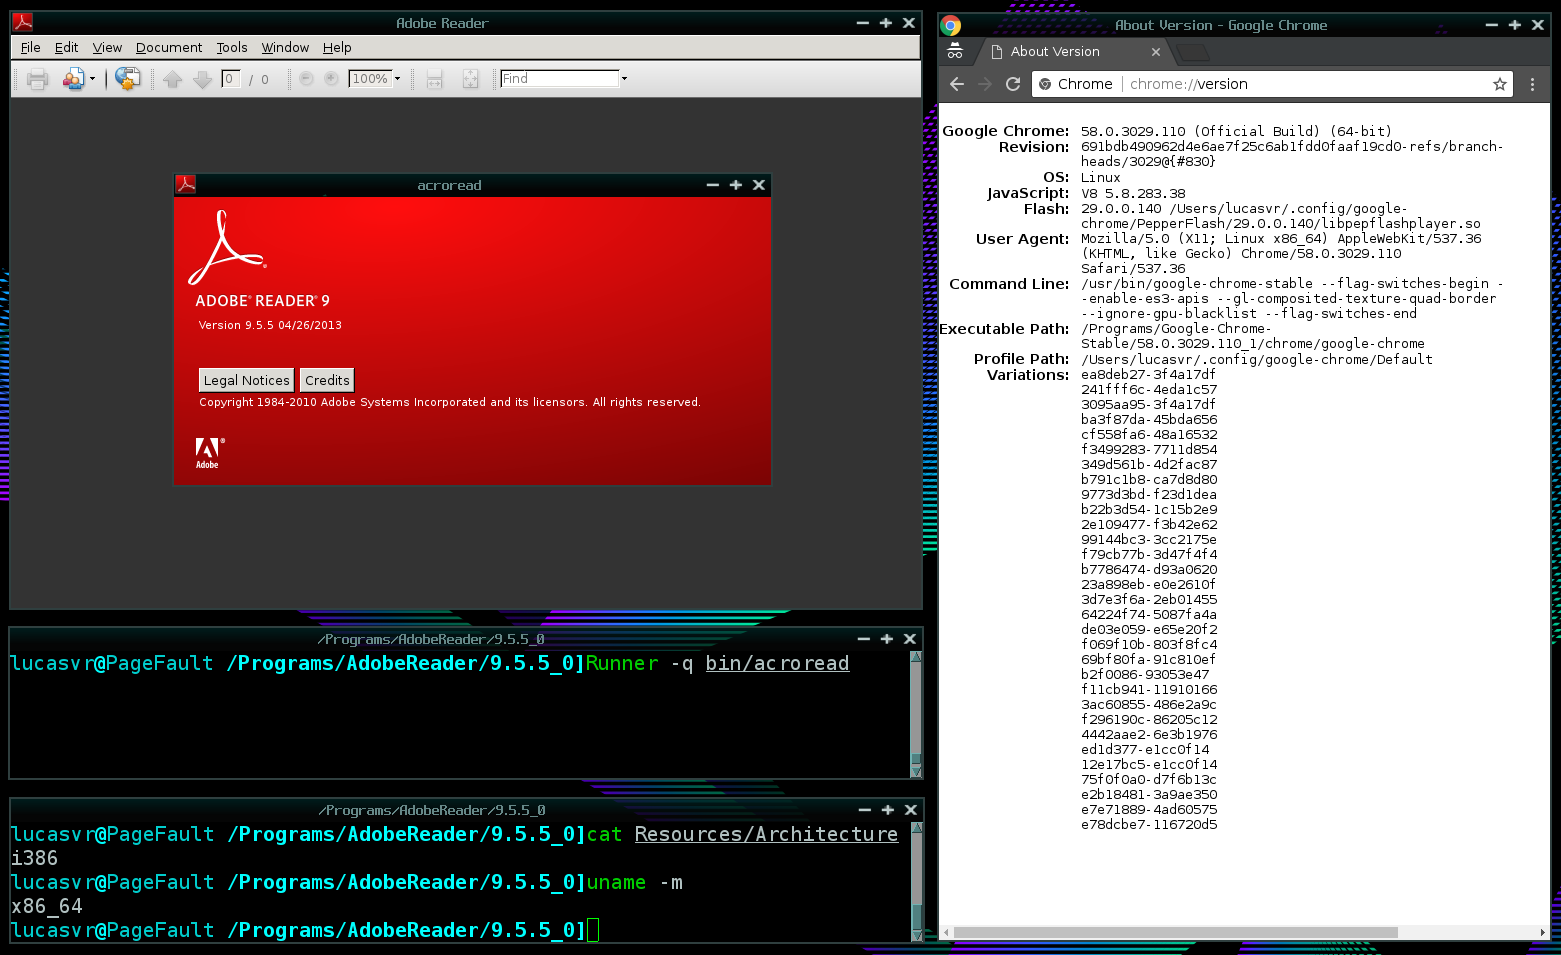
\includegraphics[width=.75\textwidth]{Runner.png}
    \caption{Using Runner to launch Adobe Reader (32-bit, from 2010) alongside Chrome (64-bit, from 2018)}
    \label{fig:runner}
\end{figure*}

\section{Conclusion}\label{sec:conclusion}
Containers are a proven technology that enables the confined execution of
processes under environments with strict security constraints and with special
needs for resource throttling. However, they impose significant administration
overhead when it comes to using them to run mundane executables that present
versioning conflicts.

We presented a container-free infrastructure that enables conflicting
dependencies to coexist in the same filesystem hierarchy and that enables
their execution through filesystem multiplexing. Our proposal extends to
packages managed by third-party software (such as those in charge of
installing programming language modules) by way of another contribution
made known in this paper: the unification of such packages under a well
structured virtual filesystem.

Because of the directory hierarchy we built our solution upon, there is
no storage waste due to the replication of dependency files. Also, through
such a hierarchy, it is possible to keep packages belonging to different
versions of the distribution installed at the same time. That enables the
realization of interesting scenarios with Runner, such as letting one run
every program ever released for the distribution with zero configuration,
as long as all related packages are uncompressed under the versioned
directory structure.

We plan on extending the engineering work we have conducted so far to
do this and that, and to continue our research on foo so that bar.

\section{Source code}
The source code of the tools presented in this paper are available at
\emph{[redacted for anonymity]}.

\bibliographystyle{ACM-Reference-Format}
\bibliography{Runner}

\end{document}
